The contribution of our proposed system will be demonstrated on \textcolor{red}{two} case studies which correspond to real problems the biochemists are currently facing. 
Then also the detailed performance analysis will be discussed.

\subsection{ Case Study 1~--~Real-time visual exploration of MD simulation}
The first case study deals with the situation when the biochemists want to visually explore the inner processes which are occurring inside the molecule. 
An example of such process can be the penetration of a small molecule (ligand) into the active site of the protein where the ligand reacts with the protein and the product of such reaction can form the basis of new chemical matters, e.g., new drugs. 
The current workflow generating the desired visual appearance of the animation showing such processes consists of many trial and error attempts which makes the whole workflow very lengthy. 
To describe it in more detail, the biochemists start in the first time step of the whole simulation and try to manually determine the best viewpoint.
As the view inside the molecule, where the processes usually occur, is crucial, they are using clip planes to enable this.
The manual setting of the clip planes introduces other possible error to the final animation.
The dynamic movements of the molecule can cause its rotation and the clip plane set in the first time step can have in the following steps completely wrong position.
When all features are set for the first frame (see Figure~\ref{fig:animation}), the biochemists use an offline rendering tool for generating the whole animation.
In this phase they do not have any control of this process so it is impossible to detect an error inside the animation and stop the generation.
These errors, such as occlusions or wrong clip plane positions, are detected when playing the final animation.
The only solution is to adjust the input settings and launch the whole process once again.
For better imagination, in case of the example video (from which Figure~\ref{fig:animation} is captured), it took two days to produce the solution which comprehensibly shows the whole process of ligand penetration to the protein active site.

\begin{figure}[htb]
  \centering
  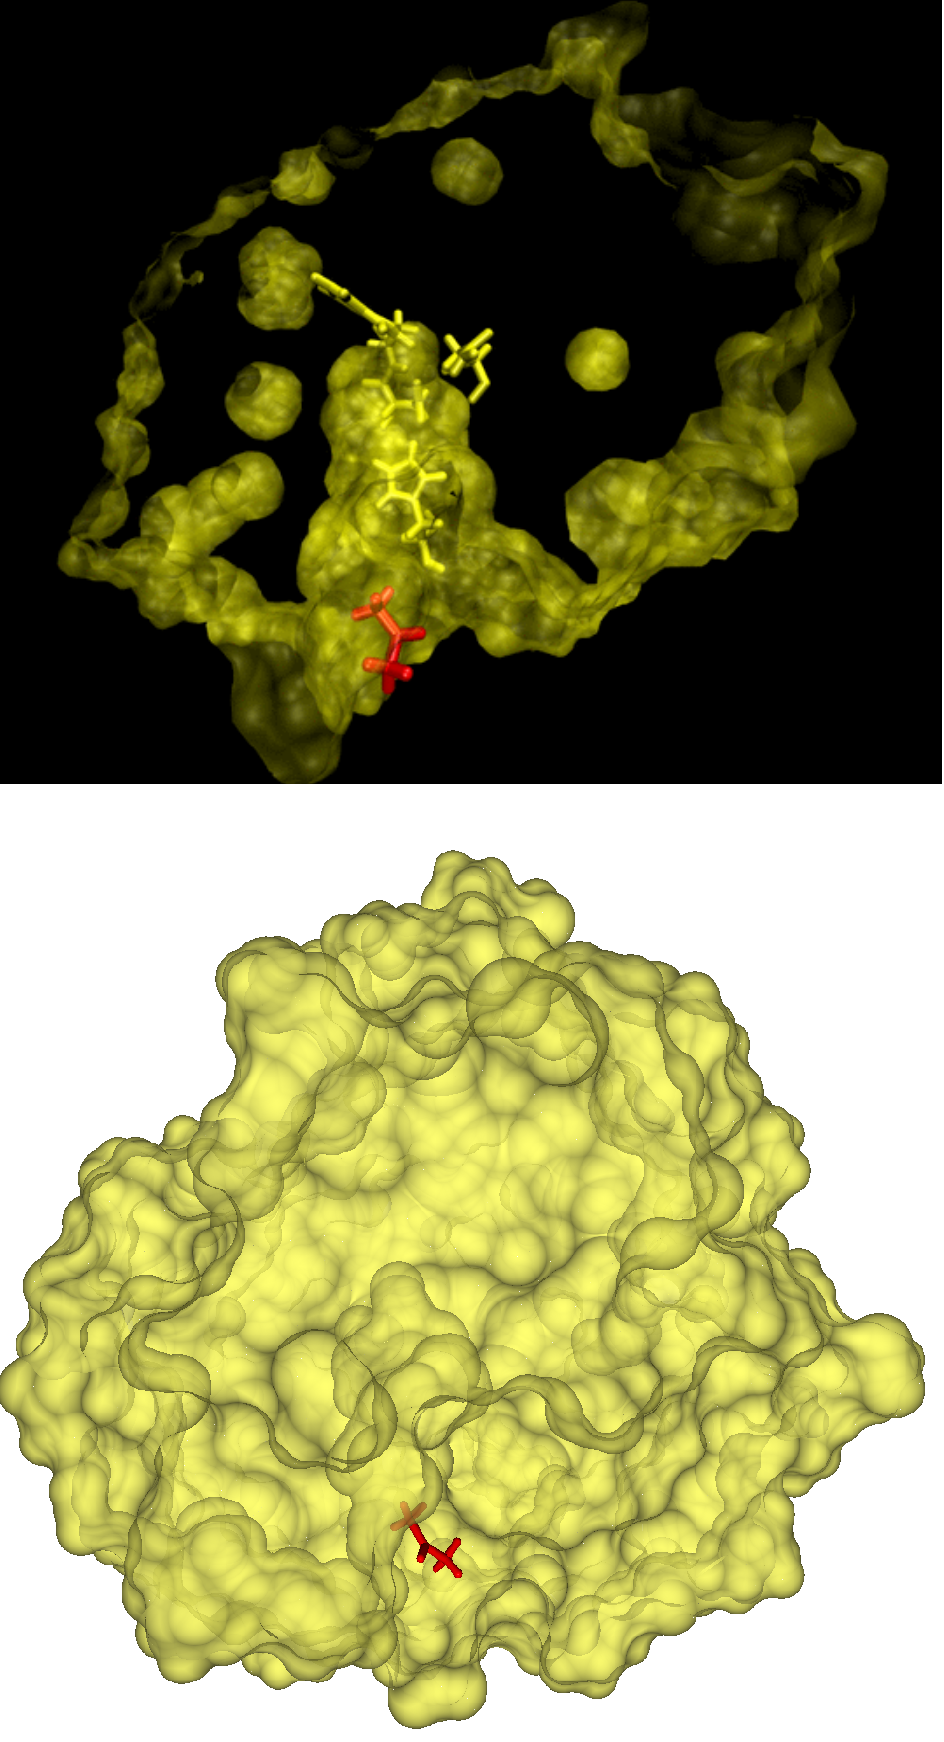
\includegraphics[width=3.3in]{image/animation.png}
  \caption{One time step from the animation aiming to show the penetration of the ligand to the protein active site. For better insight, different representations of the molecule and the ligand, surface transparency, clip plane, and different coloring was used.}
	\label{fig:animation}
\end{figure}

Our new system is able to overcome the following limitations of the above-described workflow:
\begin{itemize} 
\item The MD simulation can be observed in real time which enables the user to interactively adjust the appearance and viewpoint.
\item The highly transparent molecular surface removes the necessity of using clip planes.
\item The user had full control of the animation process so we completely remove the trial and error phase of the workflow. 
\end{itemize}

In consequence, our system enables to reach similar results in real-time. 
In one aspect it even overcomes the existing solution as the users can interactively manipulate with the scene on the fly~--~perform scene transformations, change the appearance of the protein and ligand, or change the probe size used for the generation of protein surface.

Figure \ref{fig:animation2} shows one time step of the animation generated using the same dataset as for Figure~\ref{fig:animation}.

\begin{figure}[htb]
  \centering
  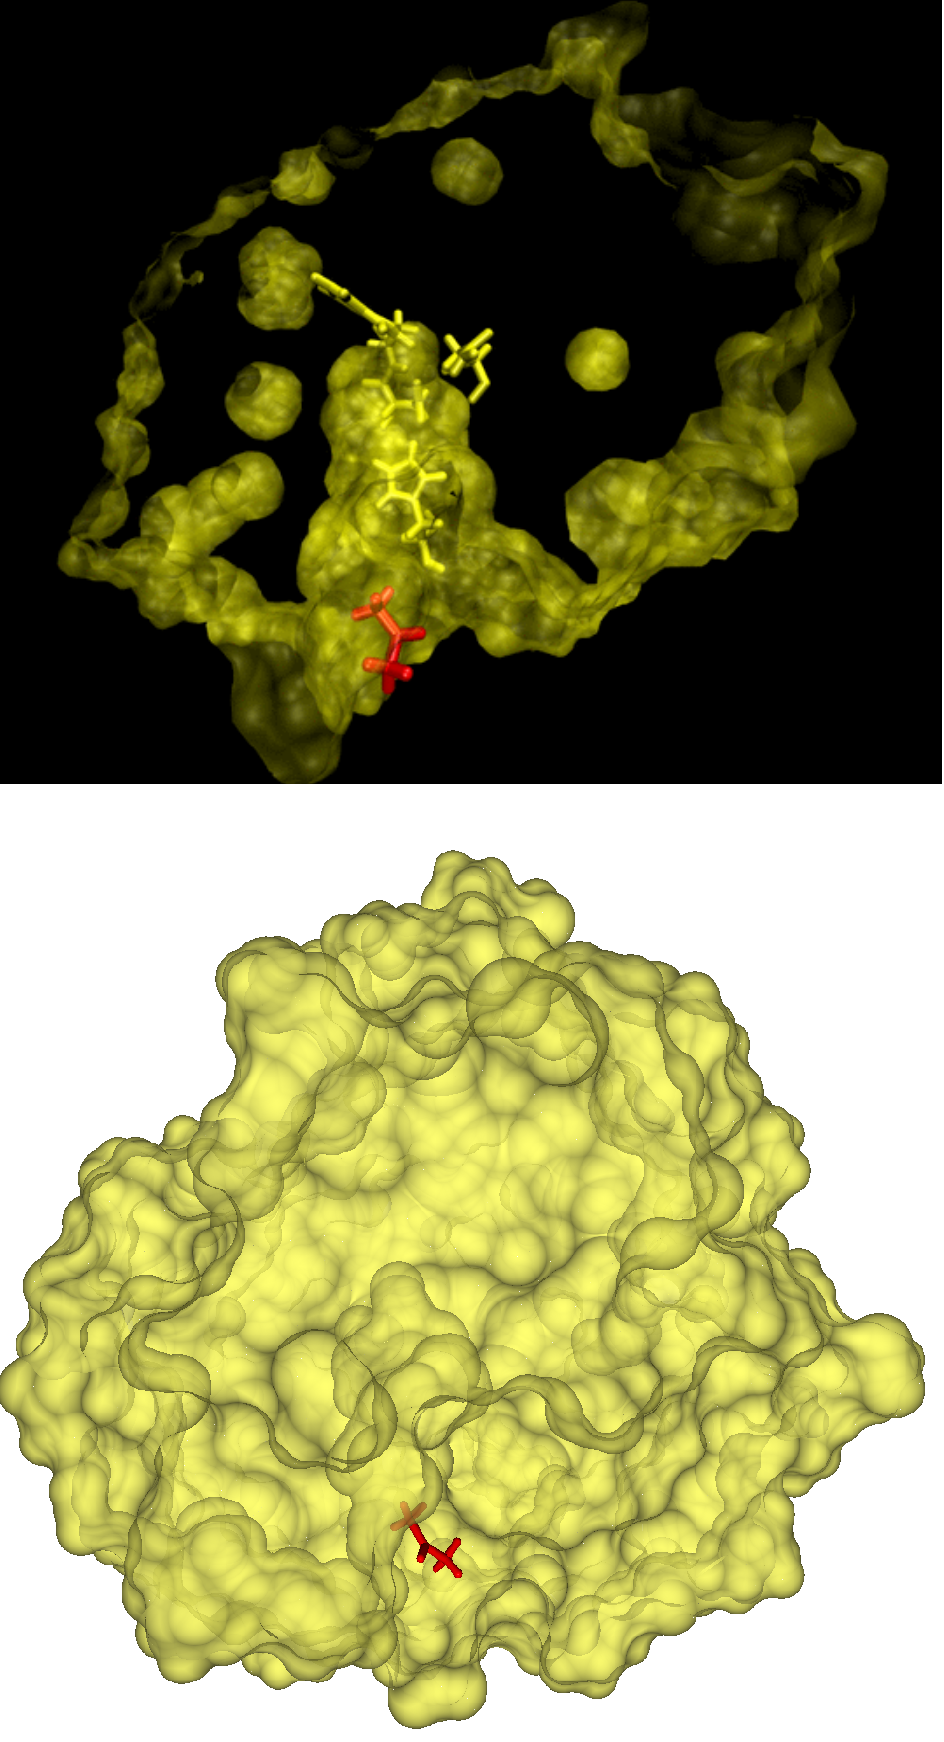
\includegraphics[width=3.3in]{image/animation.png}
  \caption{\textcolor{red}{TODO}One time step of the animation generated using our system.}
	\label{fig:animation2}
\end{figure}


\subsection{Case Study 2~--~Studying the shape of protein tunnels}
Tunnel in protein put into different organic cosolvents.

TODO

\subsection{Performance Analysis}
\label{sec:performance}

\begin{itemize}
  \item Performance analysis
  \item Pros \& cons
  \item Limits
\end{itemize}

\def\tweakedsim{\raise.17ex\hbox{$\scriptstyle\sim$}}


\begin{table}[htb]
  \caption{Performance in ms.}
  \label{tab:performance}
  \scriptsize
  \begin{center}
    \begin{tabular}{cccccc}
      MolID & Atoms & Surf & Cav & Ray & Total \\
    \hline
      1OGZ &  {\tweakedsim}1000 & 0.0 & 0.0 & 0.0 & 0.0 \\
      1VIS &  {\tweakedsim}2500 & 0.0 & 0.0 & 0.0 & 0.0 \\
      4ADJ & {\tweakedsim}10000 & 0.0 & 0.0 & 0.0 & 0.0
    \end{tabular}
  \end{center}
\end{table}
